\section{Démarche Expérimentale}

\begin{wrapfigure}{R}{0.6\linewidth}
    \centering
    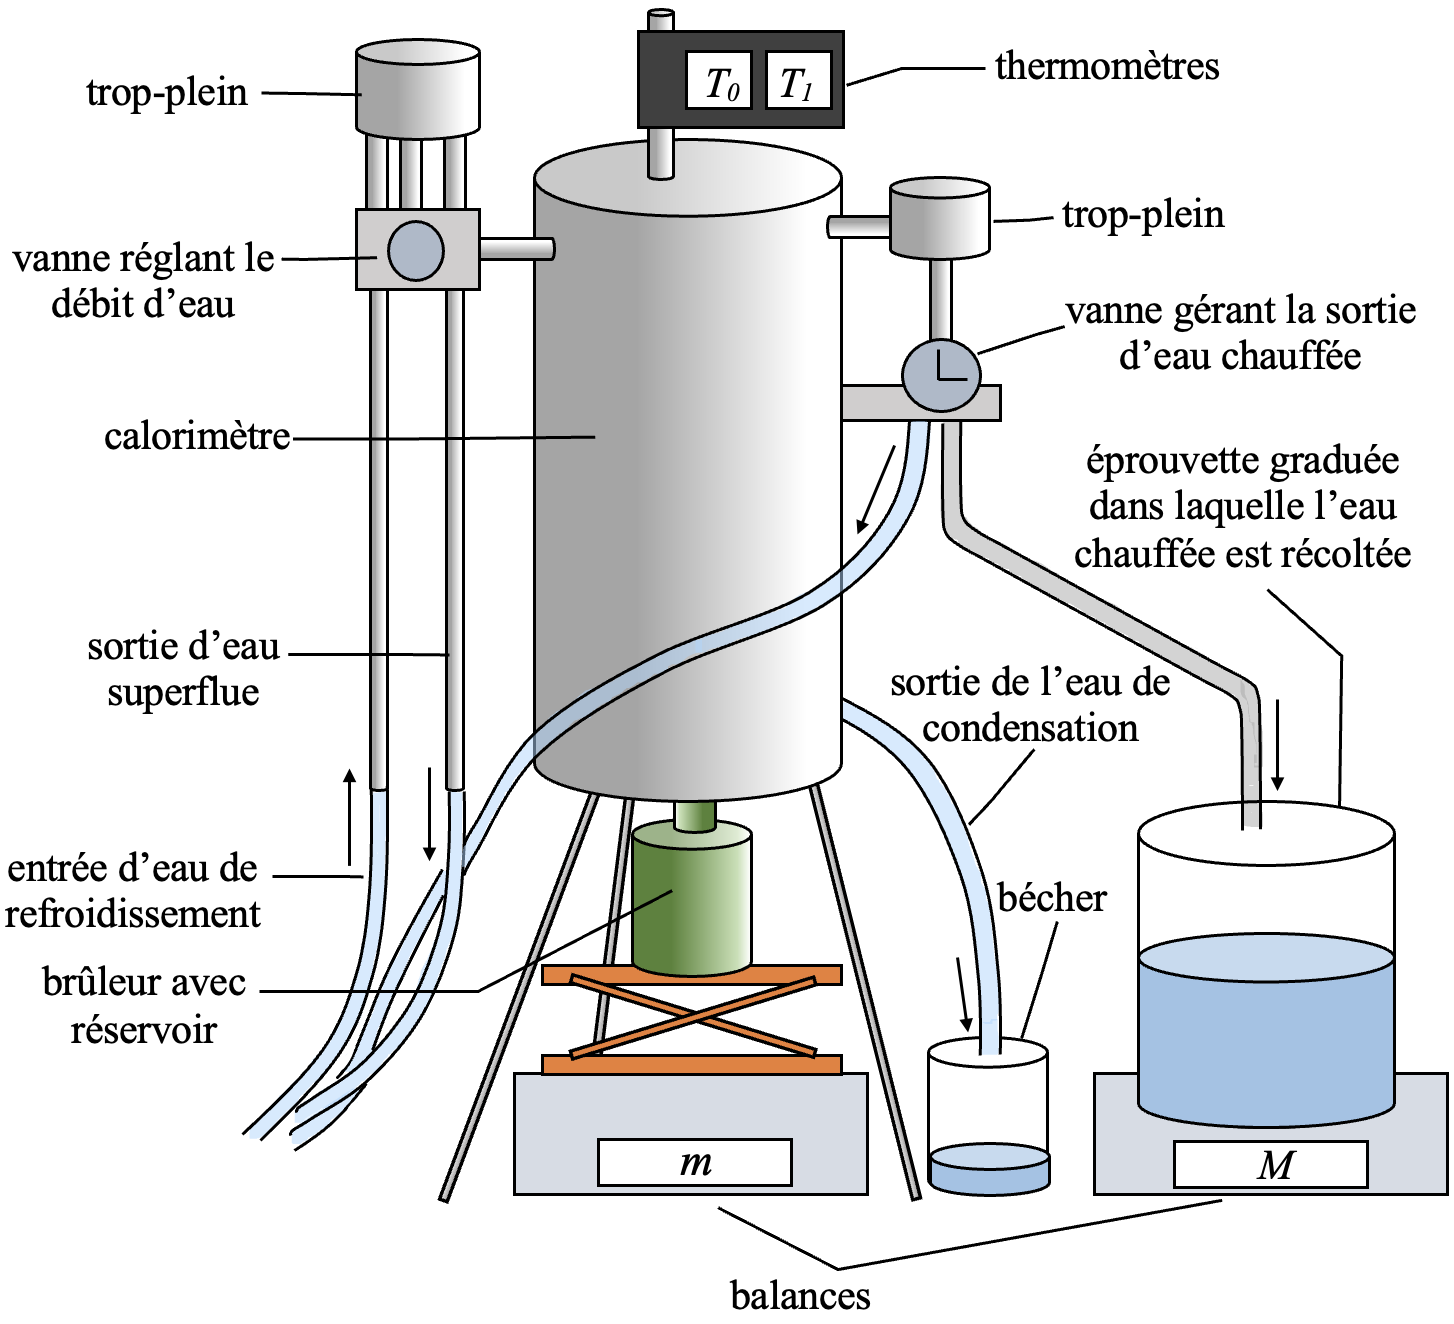
\includegraphics[width=\linewidth]{figures/montage.png}
    \caption{Montage expérimental \cite{rapport-mendels-pascaud}}
    \label{fig:montage}
\end{wrapfigure}

\paragraph*{Calorimetrie} Afin de déterminer le pouvoir calorifique des combustibles le montage à la \autoref{fig:montage} est utilisé. Le calorimettre est composé de

Le combustible est allumé (TODO: mot), chauffant le calorimettre. Les mesures s'effectuent lorsque qu'un équilibre de température est atteint, c'est à dire que l'écart entre la température d'entrée et sortie reste constant. On a alors \(\Delta U_1 = 0\). La masse d'eau \(\Delta M\) évacuée pour une certaine masse de combustible \(\Delta m\) sont mesurées à l'aide de balances digitales. L'écart de température entre l'entrée d'eau et la sortie sont relevés par des thermomètres. De plus, un bécher permet de récupérer l'eau de condensation, produite au long de l'expérience.
